Wir haben bereits ein Modell für die hypergeometrische Eben gesehen das \hyperref[hyperbolischpoincare]{Poincaré-Halbebenen-Modell}. Hier betrachtet man nun ein alternatives aber offensichtich äquivalentes Modell das \textbf{Einheitskreis-Modell} was "symmetrischer aussieht" als das Halbebenen-Modell

\begin{titleDef}{Von Poincaré zum Einheitskreis}
\label{hyperEinheitskreis}
Sei $D^2=\{(x,y)\in\Rtwo|\ x^2+y^2<1\}=\{z\in\mathbb{C}|\ \lvert z\rvert<1\}$ die \hyperref[einheitskreisscheibeoff]{offene Einheitskreisscheibe}. Die Abbildung
$$M:H^2\subset\mathbb{C}\to D^2\subset\mathbb{C};\: z\mapsto\frac{iz+1}{z+i}$$
ist eine bijektive Abbildung von der \hyperref[hyperbolischpoincare]{Poincaré-Halbebene} $H^2$ in die Einheitskreisscheibe.
\label{einheitskreismetrik}
Analog zur \hyperref[hyperbolischpoincare]{Poincaré-Halbebene} definiert man für das Einheitskreis-Modell eine \hyperref[hyperToMetrisch]{Metrik} 
$$d_h^*(z,w)=d_h(M^{-1})(z),M^{-1}(w))$$
wobei $d_h$ die Metrik der \hyperref[hyperbolischpoincare]{Poincaré-Halbebene} ist also die Länge der kürzesten Kurve die zwei Punkte verbindet.\\
Damit ist nach Konstruktion $M$ automatisch \hyperref[abstandserhaltend]{abstandserhaltend} also eine \hyperref[Isometrie]{Isometrie} also inbesondere eine \hyperref[moebiustrans]{Möbiustransformation} $T_A$ für
$$A=\begin{pmatrix}
	i&1\\1&i
\end{pmatrix}$$
\end{titleDef}

\begin{titleDef}{Metrik des Einheitskreismodells}
\label{metrikEinheitskreis}
$d_h^*$ ist die Längenmetrik die von der \hyperref[riemannMetrik]{Riemmanschen Metrik}
$$(g_{ij}(z))=\left(\frac{4\delta_{ij}}{(1-\lvert z\rvert^2)^2}\right)$$
auf $D^2$ induziert wird. Also ist insbesondere $(D^2,d_h^*)$ ein \hyperref[MetrischerRaum]{Metrischer Raum}.\par
Für $0\leq r<1$ gilt:
$$d_h^*(0,ri)=\ln\left(\frac{1+r}{1-r}\right)$$
\end{titleDef}

\begin{titleDef}{Isometrien des metrischen Raums $(D^2,d_h^*)$}
Neben den \hyperref[moebiustrans]{Möbiustransformationen} $T_A$ die bekannt sind, sind die Rotationen um $0\in D^2$ \hyperref[Isometrie]{Isometrien} im Einheitskreismodell $(D^2,d_h^*)$
\end{titleDef}

\newpage
\begin{titleDef}{Geodätische Linien}
\label{geodaetischeLinienEinheitskreis}
\hyperref[geodaetischeLinie]{Geodätische Linien} also kürzeste Verbindungsstrecken im Einheitskreismodell $(D^2,d_h^*)$ sind :
\begin{itemize}
	\item (geeignet parametrisierte) Geraden durch 0
	\item Alle anderen \hyperref[geodaetischeLinie]{Geodätische Linien} sind euklidische Kreise, die den Einheitskreis orthogonal schneiden.
\end{itemize}
\begin{figure}[h]
	\centering
	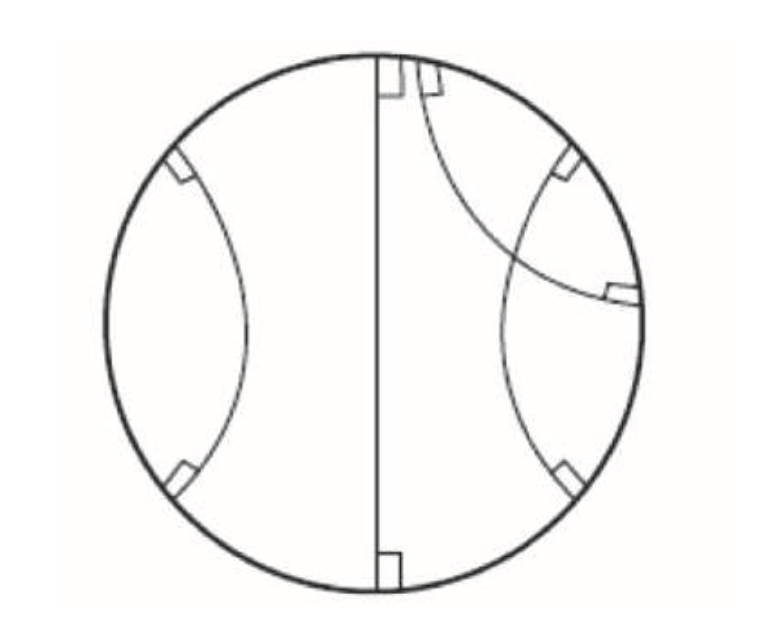
\includegraphics[width=200px]{Bilder/GeodaetischeEinheitskreis}
	\label{geodaetischeHyperEinheitGrafik}
\end{figure}\par
Der \hyperref[unendlicherRand]{unendliche Rand} $\partial_\infty D^2=\mathbb{R}\cup\{\infty\}$ von $D^2$ ist gerade der Einheitskreis $S_1^1$

\end{titleDef}

\begin{titleDef}{hyperbolische Kreis}
\label{hyperKreis}
Der \textbf{hyperbolische Kreis} $S_\varrho(0)$ in $D^2$ mit Zentrum 0 und hyperbolischen Radius (also der Radius gemessen gemäß der \hyperref[hyperLaenge]{hyperbolischen Länge} $L_{h^*}$) ist der euklidische Kreis $S_1^1$ um 0 mit euklidischen Radius r, wobei
$$\varrho=2arctan(r)\Longleftrightarrow r=\tanh(\frac{\varrho}{2})$$
insbesondere gilt $\varrho\to\infty$ für $r\to 1$.\par
Die \hyperref[hyperLaenge]{hyperbolische Länge} des hyperbolischen Kreises $S_\varrho(0)$ ist:
$$L_{h^*}(S_\varrho(0))=2\pi\sinh(\varrho)=2\pi\frac{1}{2}(e^\varrho-e^{-\varrho})\: (\sim\pi e^\varrho \text{ für großes }\varrho)$$
\end{titleDef}

\begin{titleDef}{Gauß-Krümmung}
\label{gausskruemmungEinheitskreis}
Die \hyperref[gausskruemmung]{\textbf{Gauß-Krümmung}} einer hyperbolischen Ebene also von $H^2$ bzw $D^2$ ist konstant $K(p)\cong-1$\par
Reskaliert man die \hyperref[hyperToMetrisch]{hyperbolische Metrik} $d_{h^*}$, setzt also $d_{\tilde{h}}=\lambda d_{h^*}$ für $\lambda\in\mathbb{R}, \lambda>0$ so gilt für die Länge des \hyperref[hyperKreis]{hyperbolischen Kreises}:
$$L_{\tilde{h}}(S_\varrho(0))=2\pi\sinh(\frac{\varrho}{\lambda})$$
daraus folgt für die \hyperref[gausskruemmung]{Gauß-Krümmung} von $(D^2,d_{\tilde{h}})$:
$$K_{\tilde{h}}(p)=-\frac{1}{\lambda^2}=\text{konstant}$$
Durch passende Reskalierungen erhält man also Modelle der hypergeometrischen Ebene mit beliebiger, konstanter negativer Krümmung.\par
Abschließend erhält man also nun für jede reelle Zahl $\alpha\in\mathbb{R}$ eine \hyperref[regFlaeche]{reguläre Fläche} bzw 2-dimensionale \hyperref[diffMannigfaltigkeit]{differenzierbare Mannigfaltigkeit} die genau konstante Krümmung $\alpha$ hat.
\begin{itemize}
	\item Für $\alpha>0$ die \hyperref[ndimsphere]{2-Sphäre} $S_{\frac{1}{\sqrt{\alpha}}}^2$ mit Radius $R=\frac{1}{\sqrt{\alpha}}$
	\item Für $\alpha=0$ die euklidische Ebene
	\item Für $\alpha<0$ die \hyperref[hyperEinheitskreis]{Einheitskreisscheibe} $D^2$ (bzw das isometrische Modell $H^2$ der \hyperref[hyperbolischpoincare]{Poincaré-Halbebene}) mit der Metrik $\frac{1}{\sqrt{\alpha}}d_{h^*}$ bzw $\frac{1}{\sqrt{\alpha}}d_{h}$
\end{itemize}
\end{titleDef}